
\begin{frame}[fragile]{Cover tree performance comparisons}
\begin{center}
\graphicspath{{covertree/paperimg/}}
\input{slides/covertree/paperimg/parallel}
\definecolor{colorOrig}{RGB}{102,51,0}
\definecolor{colorMlpack}{RGB}{204,153,0}
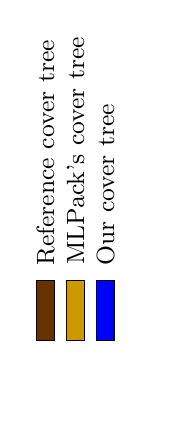
\begin{tikzpicture}
    \node[draw,fill=colorOrig,minimum width=0.05in,minimum height=0.3in] at (0,0) {};
    \node at (0,0.79in) {\small\rotatebox{90}{Reference cover tree}};
    \node[draw,fill=colorMlpack,minimum width=0.05in,minimum height=0.3in] at (0.15in,0) {};
    \node at (0.15in,0.80in) {\small\rotatebox{90}{MLPack's cover tree}};
    \node[draw,fill=blue,minimum width=0.05in,minimum height=0.3in] at (0.3in,0) {};
    \node at (0.3in,0.63in) {\small\rotatebox{90}{Our cover tree}};
    \node[minimum width=0.05in,minimum height=0.3in] at (0.45in,0) {};
    \node at (0.45in,0.61in) {\small\rotatebox{90}{}};
    \node at (0,-0.475in) {};
\end{tikzpicture}
\end{center}

\vspace{0.1in}
Experiments run on an Amazon AWS instance with 16 true cores
\end{frame}
